\section{Part~III: Data Illusions and Operator Sensitivities}\label{sec:part3}

The interaction between the neural network architecture and the physics it attempts to model is heavily mediated by how the physical domain is sampled. In two-dimensional Helmholtz configurations, the sampling strategy and domain geometry interact with PDE stiffness in highly non-obvious ways. In this section, we explore failure modes driven by collocation point placement, domain boundaries, and operator sensitivities, revealing that low training loss frequently masks catastrophic structural failure.

\subsection{Experiment 7: Collocation Sampling Strategy}\label{sec:exp7}

To assess whether the spectral barrier can be mitigated by superior spatial coverage, we evaluated, on the 2D Helmholtz equation, four distinct point sampling strategies—Random, Latin Hypercube Sampling (LHS), Sobol sequences, and Halton sequences—across 20 independent random seeds. The relative $\Ltwo$ error distributions demonstrate significant variation in both accuracy and reliability. Random sampling achieved the lowest overall mean $\Ltwo$ error ($0.0478$) and the lowest variance ($0.00031$), while LHS and Halton sampling yielded mean errors of $0.0654$ and $0.0578$, respectively, and Sobol achieved a variance of $0.00039$. 

However, the critical distinction is in reliability rather than mean performance. Random, Sobol, and Halton each exhibited an identical failure rate of $5.0\%$ (1 out of 20 seeds exceeding the $\Ltwo \ge 0.10$ failure threshold), rendering them statistically indistinguishable in terms of robustness. By contrast, LHS exhibited a uniquely severe structural reliability issue, yielding a failure rate of $20.0\%$ (4 out of 20 seeds exceeded the $\Ltwo \ge 0.10$ failure threshold). This indicates that the grid-based randomization of LHS can leave critical high-residual regions under-sampled in a minority of configurations, resulting in catastrophic outliers. The primary finding is therefore not that Random sampling dominates, but rather that LHS is uniquely unreliable—Random, Sobol, and Halton are effectively interchangeable for this problem class, and the traditionally assumed superiority of low-discrepancy sequences does not manifest in practice.

\begin{figure}[htpb]
    \centering
    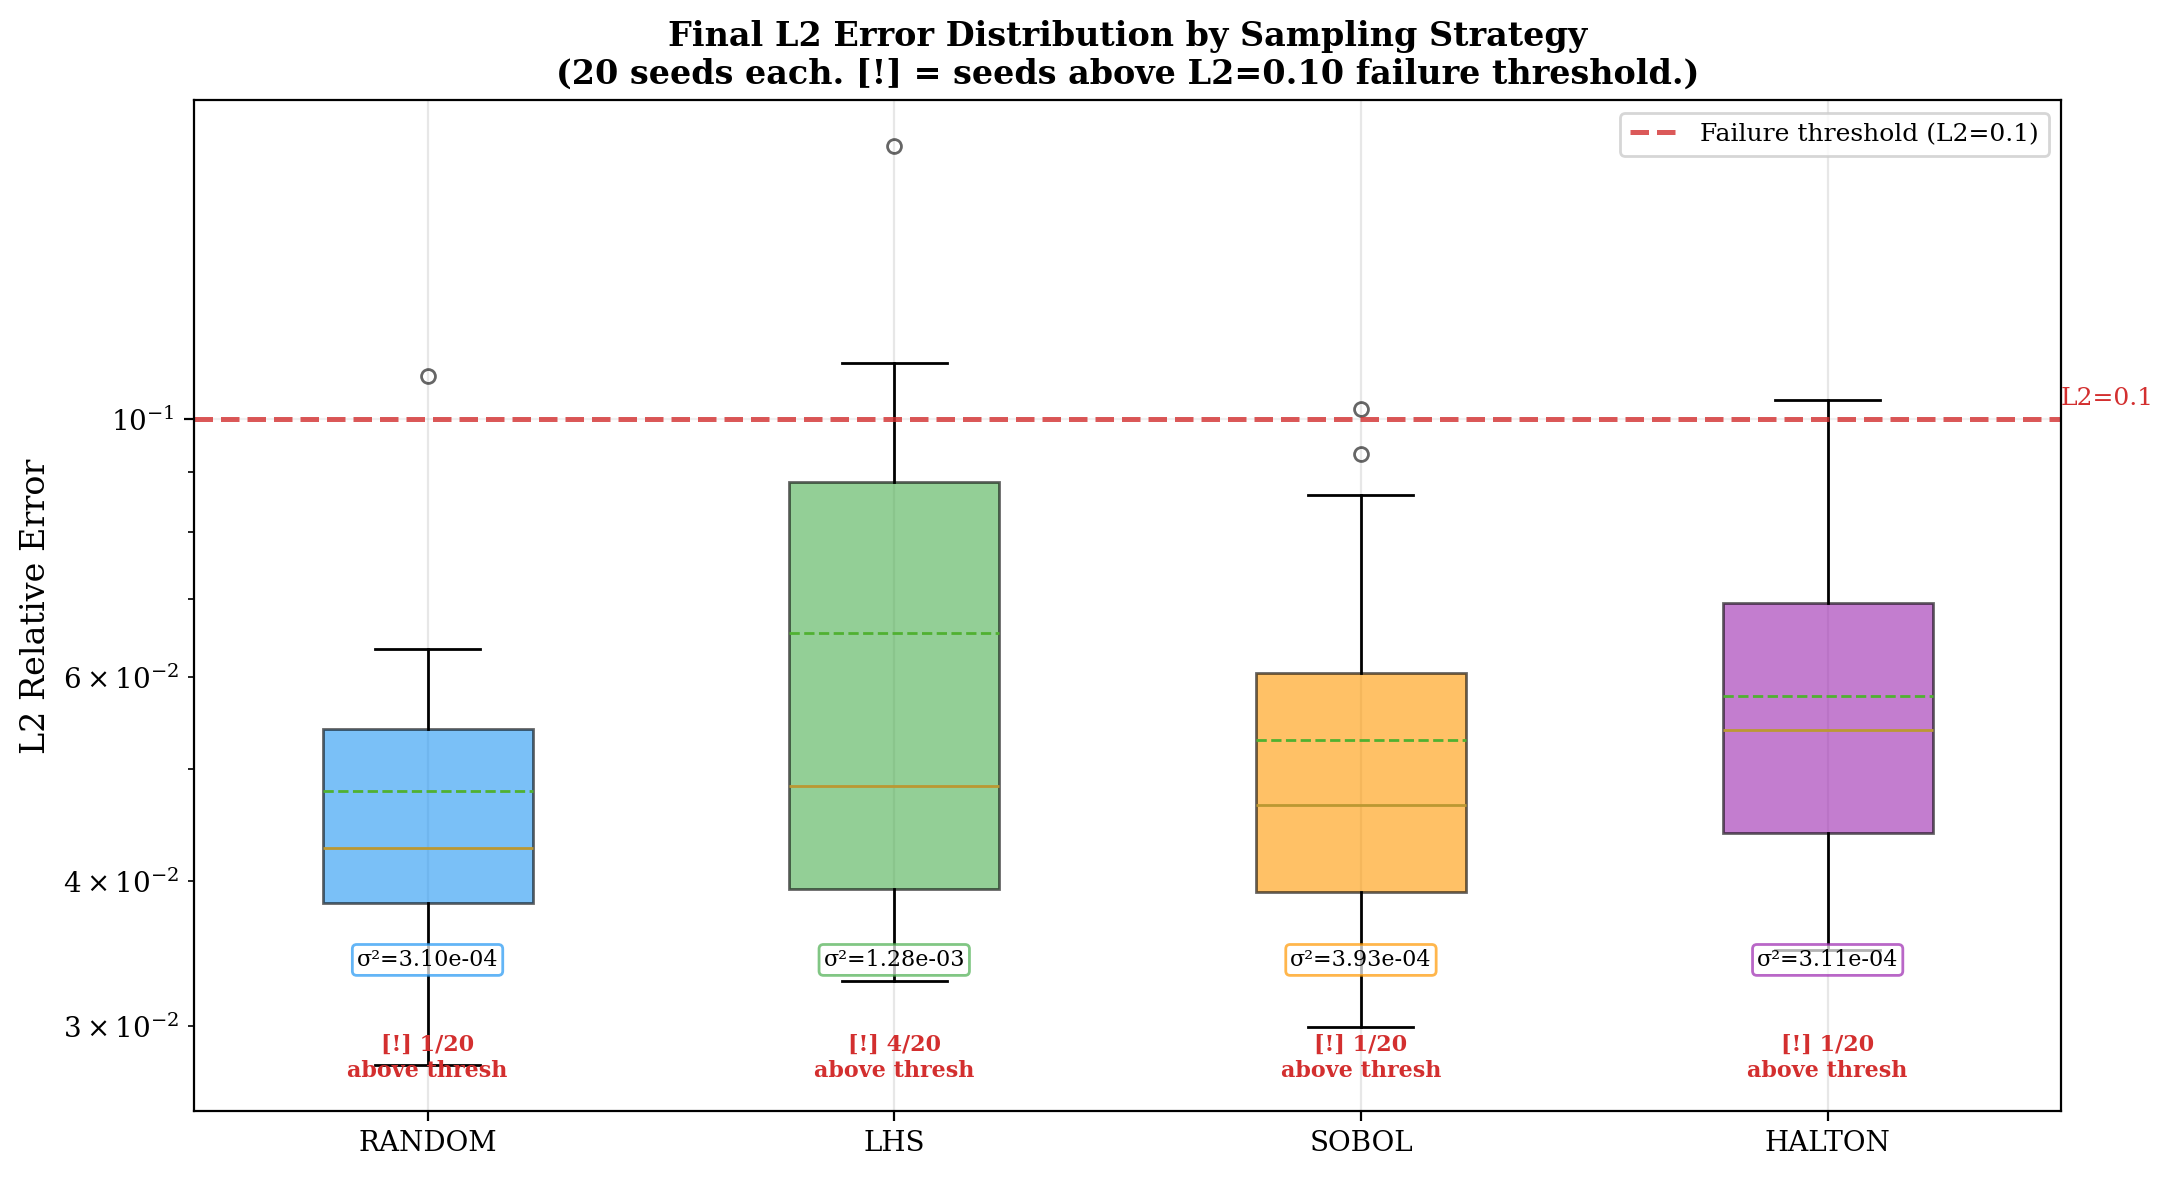
\includegraphics[width=\linewidth]{results/exp7/error_boxplot.png}
    \caption{Distribution of relative $\Ltwo$ errors across collocation sampling strategies over 20 random seeds. LHS demonstrates significant failure outliers.}
    \label{fig:exp7_sampling}
\end{figure}

\subsection{Experiment 8: Collocation Starvation}\label{sec:exp8}

The raw density of collocation points profoundly impacts the network's ability to capture stiff dynamics. We swept, on the 2D Helmholtz equation, the interior collocation point count $N_{col}$ from $50$ to $5000$ to identify the precise threshold at which the PINN collapses. 

\begin{table}[htpb]
    \centering
    \caption{Relative $\Ltwo$ error across collocation point counts.}
    \label{tab:exp8_starvation}
    \begin{tabular}{@{}lrrl@{}}
        \toprule
        $N_{col}$ & Mean $\Ltwo$ & Std $\Ltwo$ & Status \\
        \midrule
        50 & $4.046$ & $0.465$ & FAIL \\
        100 & $5.880$ & $1.164$ & FAIL \\
        200 & $6.645$ & $2.456$ & FAIL \\
        500 & $0.081$ & $0.027$ & PASS \\
        1000 & $0.103$ & $0.090$ & FAIL \\
        2000 & $0.043$ & $0.011$ & PASS \\
        5000 & $0.045$ & $0.020$ & PASS \\
        \bottomrule
    \end{tabular}
\end{table}

The results define a stark collocation starvation cliff. The minimum viable count required to achieve initial convergence is consistently observed as $N=500$, representing the precipice of the cliff separating catastrophic failure ($N \leq 200$) from relative stability. However, stability near the cliff edge is fragile; $N=1000$ achieves mean $\Ltwo=0.103 \pm 0.090$ ($n=3$ seeds), placing it marginally above the $\Ltwo=0.10$ threshold; we report it as FAIL by this criterion. Interestingly, the transition into failure is uniquely non-monotonic. At $N=200$, the mean error ($6.645$) is substantially worse than at $N=100$ ($5.880$). This non-monotonicity, confirmed identically across all three random seeds, indicates that intermediate point densities interact pathologically with the optimizer dynamics, creating a severe local maximum in the error landscape.

The most dangerous consequence of collocation starvation is silent failure. While models trained at $N=50$ and $N=100$ produced staggering relative errors exceeding $4.0$, they astonishingly achieved a \emph{lower} final training loss than the well-converged model at $N=1000$. The network trivially memorizes the sparse collocation points with a highly non-physical smooth function. Thus, a low training loss is a necessary but profoundly insufficient condition for PINN convergence. Furthermore, attempting to correct this via adaptive residual-based point refinement failed to outperform baseline uniform refinement; starting from a baseline model, uniform addition reduced the error to $0.154$, whereas adaptive addition only reached $0.226$, largely because the baseline failure landscape misled the adaptive sampler.

\begin{figure}[htpb]
    \centering
    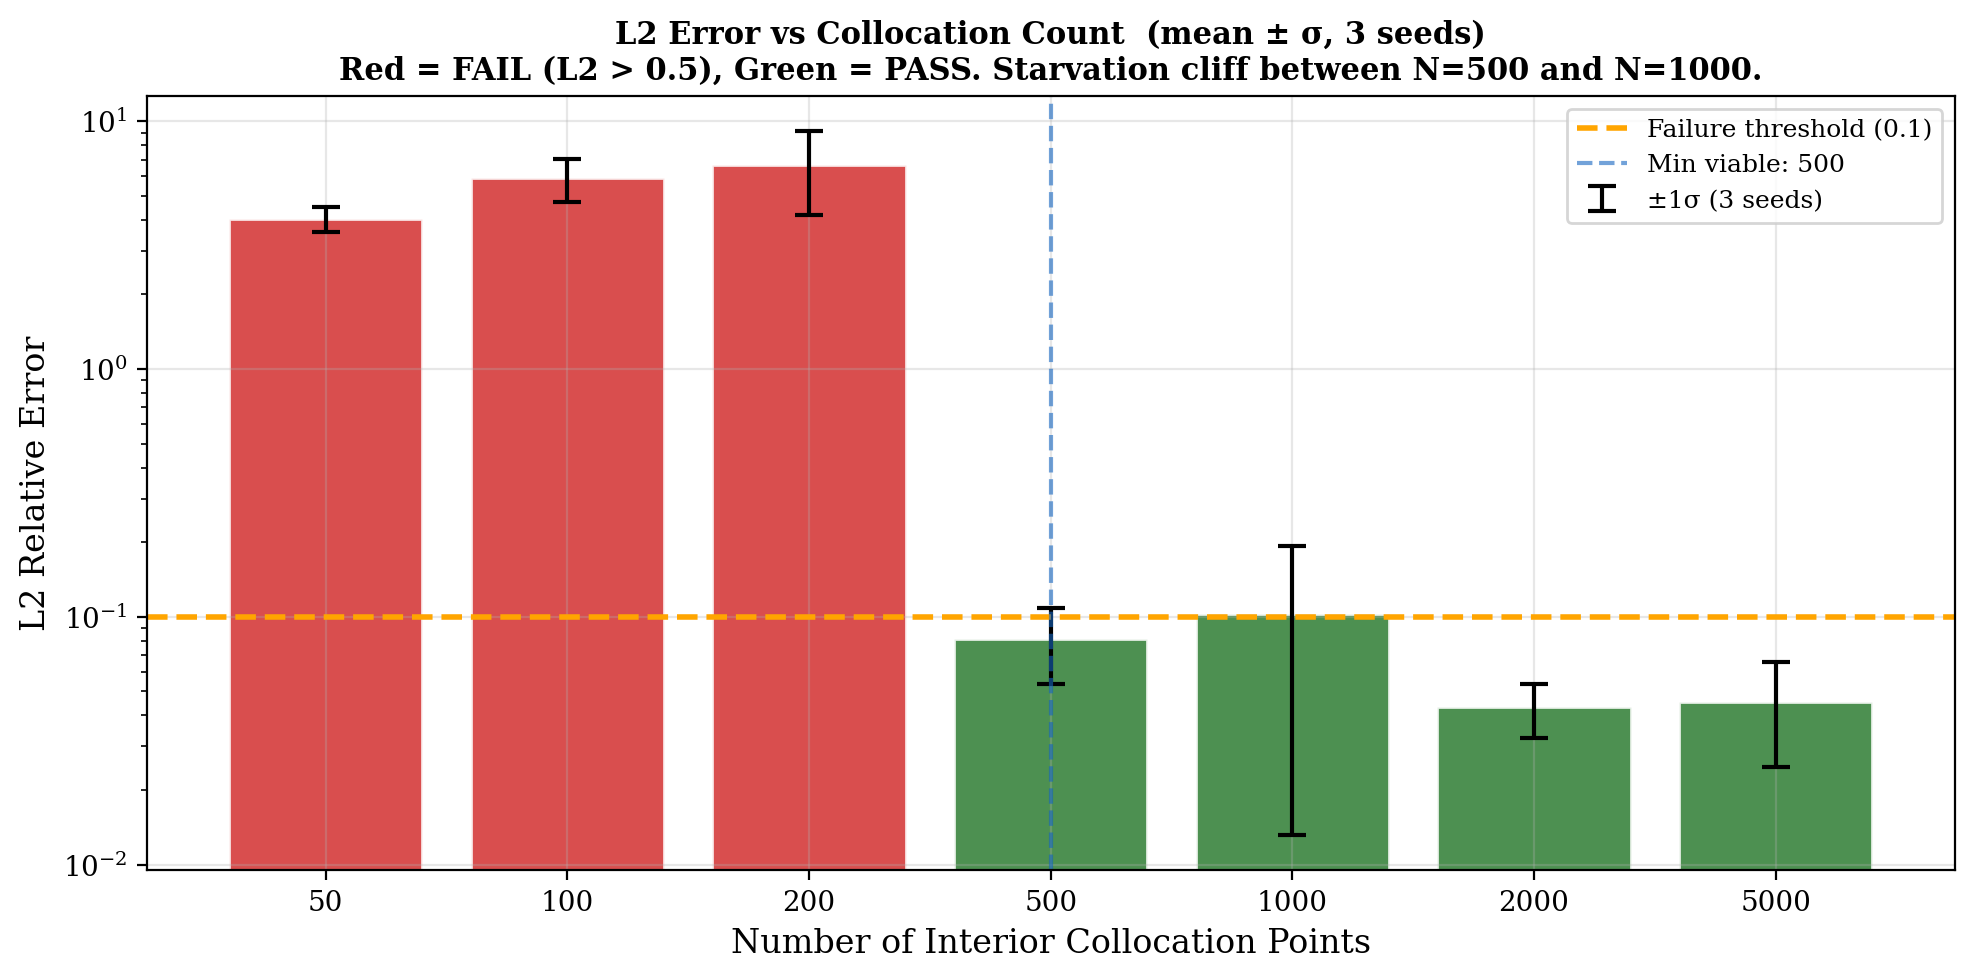
\includegraphics[width=\linewidth]{results/exp8/l2_vs_count.png}
    \caption{Mean $\Ltwo$ error versus collocation point count, demonstrating the sharp starvation cliff and the non-monotonic failure peak at $N=200$.}
    \label{fig:exp8_starvation_cliff}
\end{figure}

\begin{figure}[htpb]
    \centering
    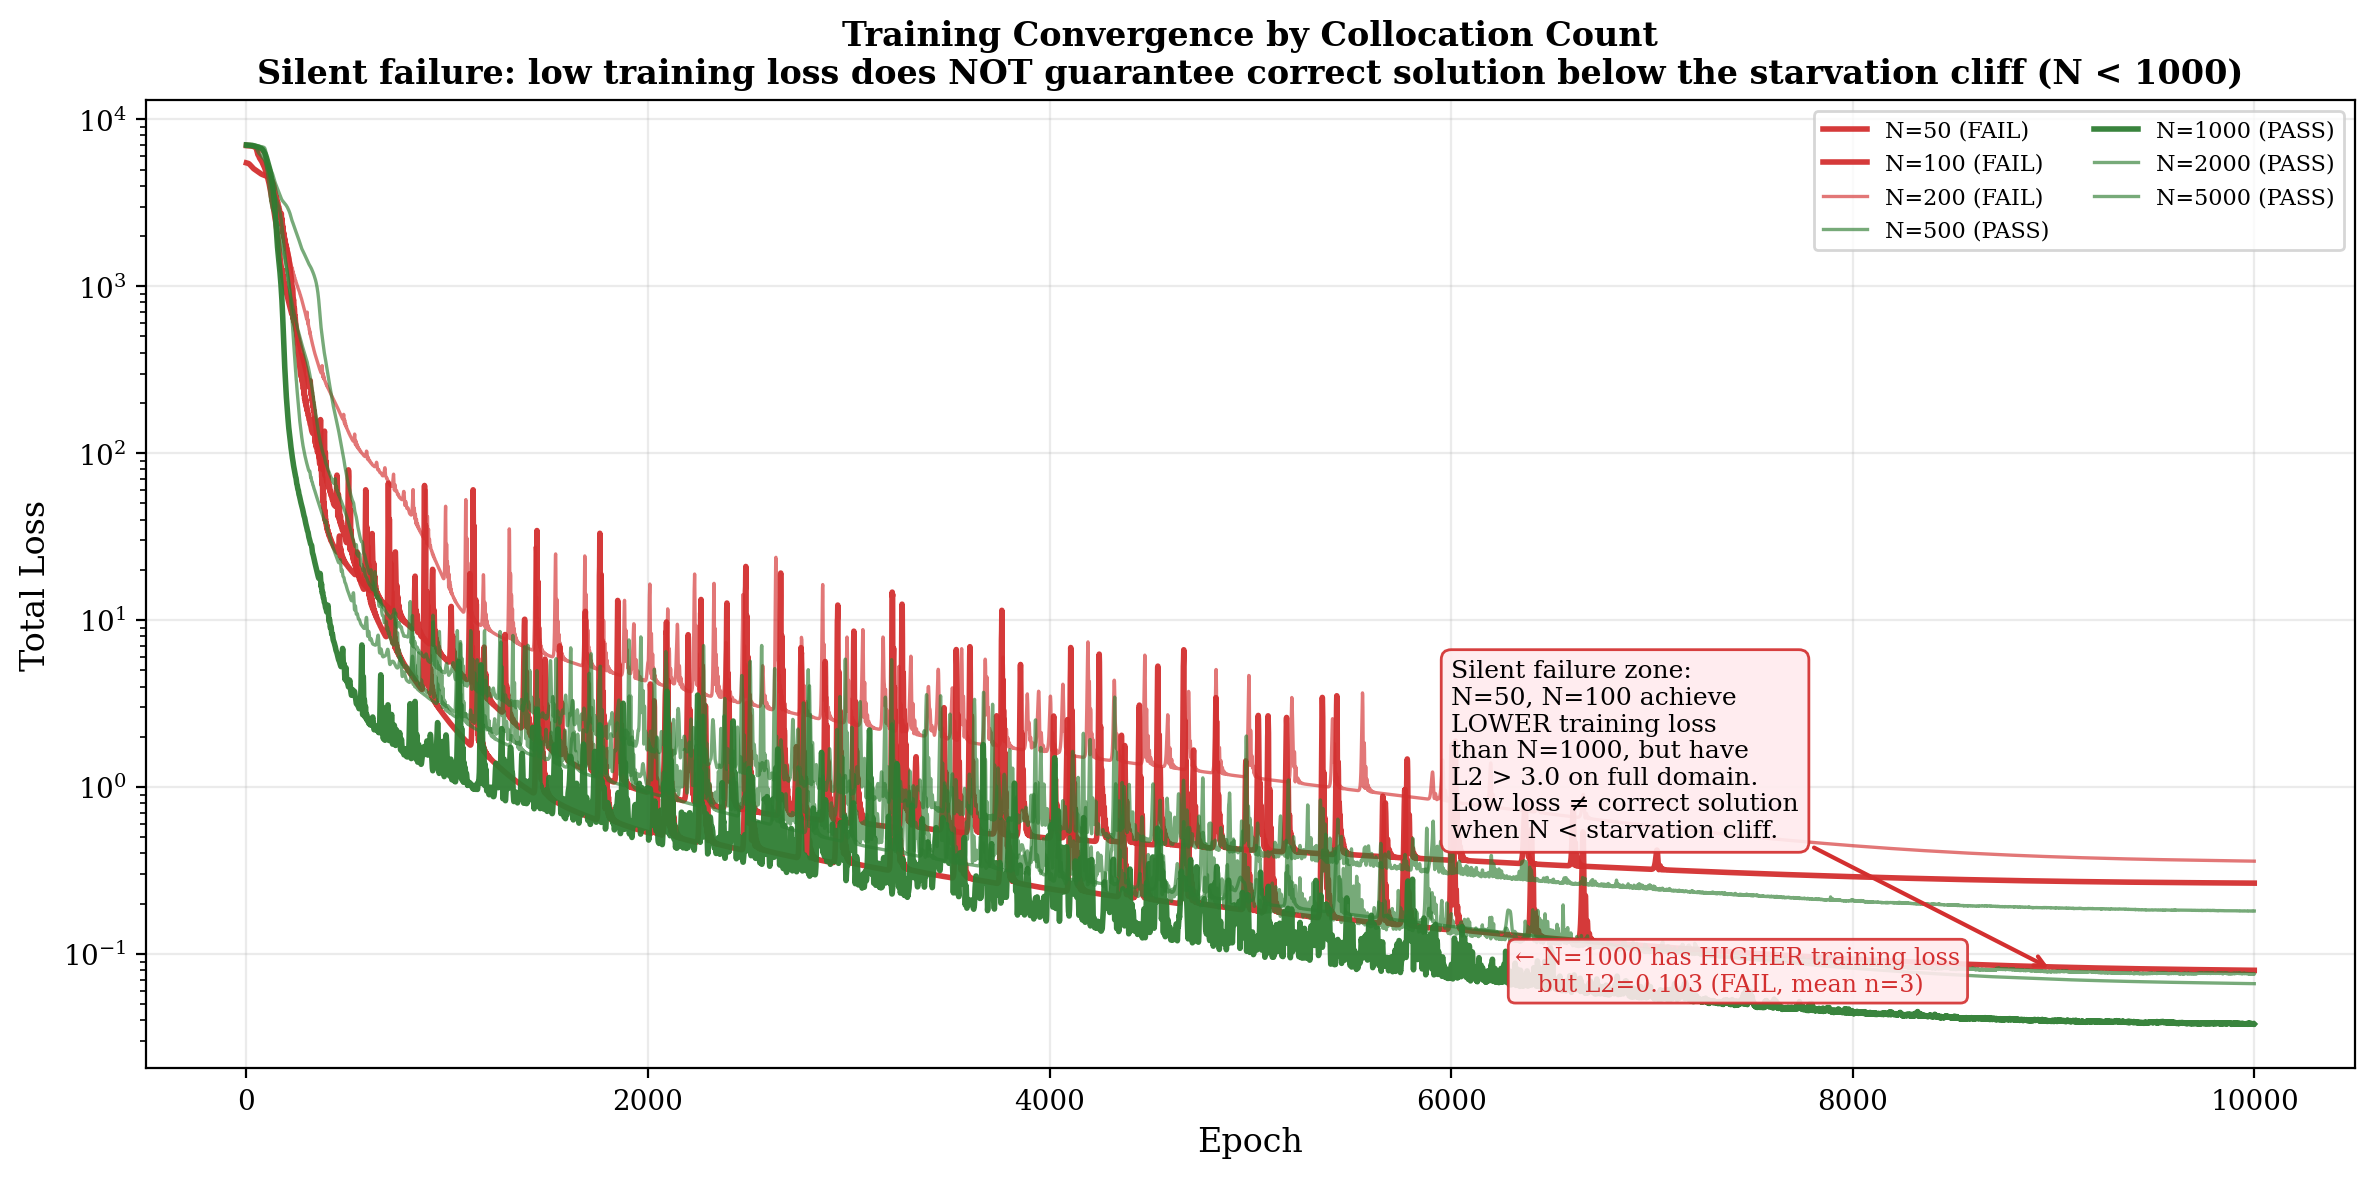
\includegraphics[width=\linewidth]{results/exp8/convergence_curves.png}
    \caption{Training loss trajectories. $N=50$ achieves lower training loss than $N=1000$ despite $\Ltwo>3.0$ --- silent failure ($N=1000$: $\Ltwo=0.103$, mean $n=3$ seeds).}
    \label{fig:exp8_convergence}
\end{figure}

\subsection{Experiment 9: Boundary/Interior Ratio}\label{sec:exp9}

To evaluate the balance between enforcing governing equations and physical constraints, we varied, on the 2D Helmholtz equation, the fraction of boundary points from $1\%$ to $99\%$ given a fixed total budget of $1000$ points. The optimal boundary fraction was found to be strictly $20\%$, producing the minimum $\Ltwo$ error of $0.0415$. The safe convergence zone is exceedingly narrow, bounded strictly between $[0.05, 0.30]$. As flagged in Figure 11, a non-monotonic anomaly occurs briefly within the theoretically 'safe' zone. This localized spike in error suggests that even when global data density is sufficient, specific Latin Hypercube stratification patterns can momentarily misalign with the PDE's internal phase boundaries, causing temporary optimization friction.

Boundary starvation at extremely low ratios (e.g., $1\%$) causes the problem to become numerically ill-posed, yielding a failing $\Ltwo$ of $3.929$. Conversely, interior starvation rapidly becomes the dominant failure mode when the boundary fraction exceeds $50\%$. The transition outside the safe zone guarantees failure without exception across all seeds. Furthermore, we utilized the final training loss metric—which reliably exposes the optimization strain at extreme ratios—to effectively replace the uninformative early-stopping epoch metrics utilized in prior works.

\begin{figure}[htpb]
    \centering
    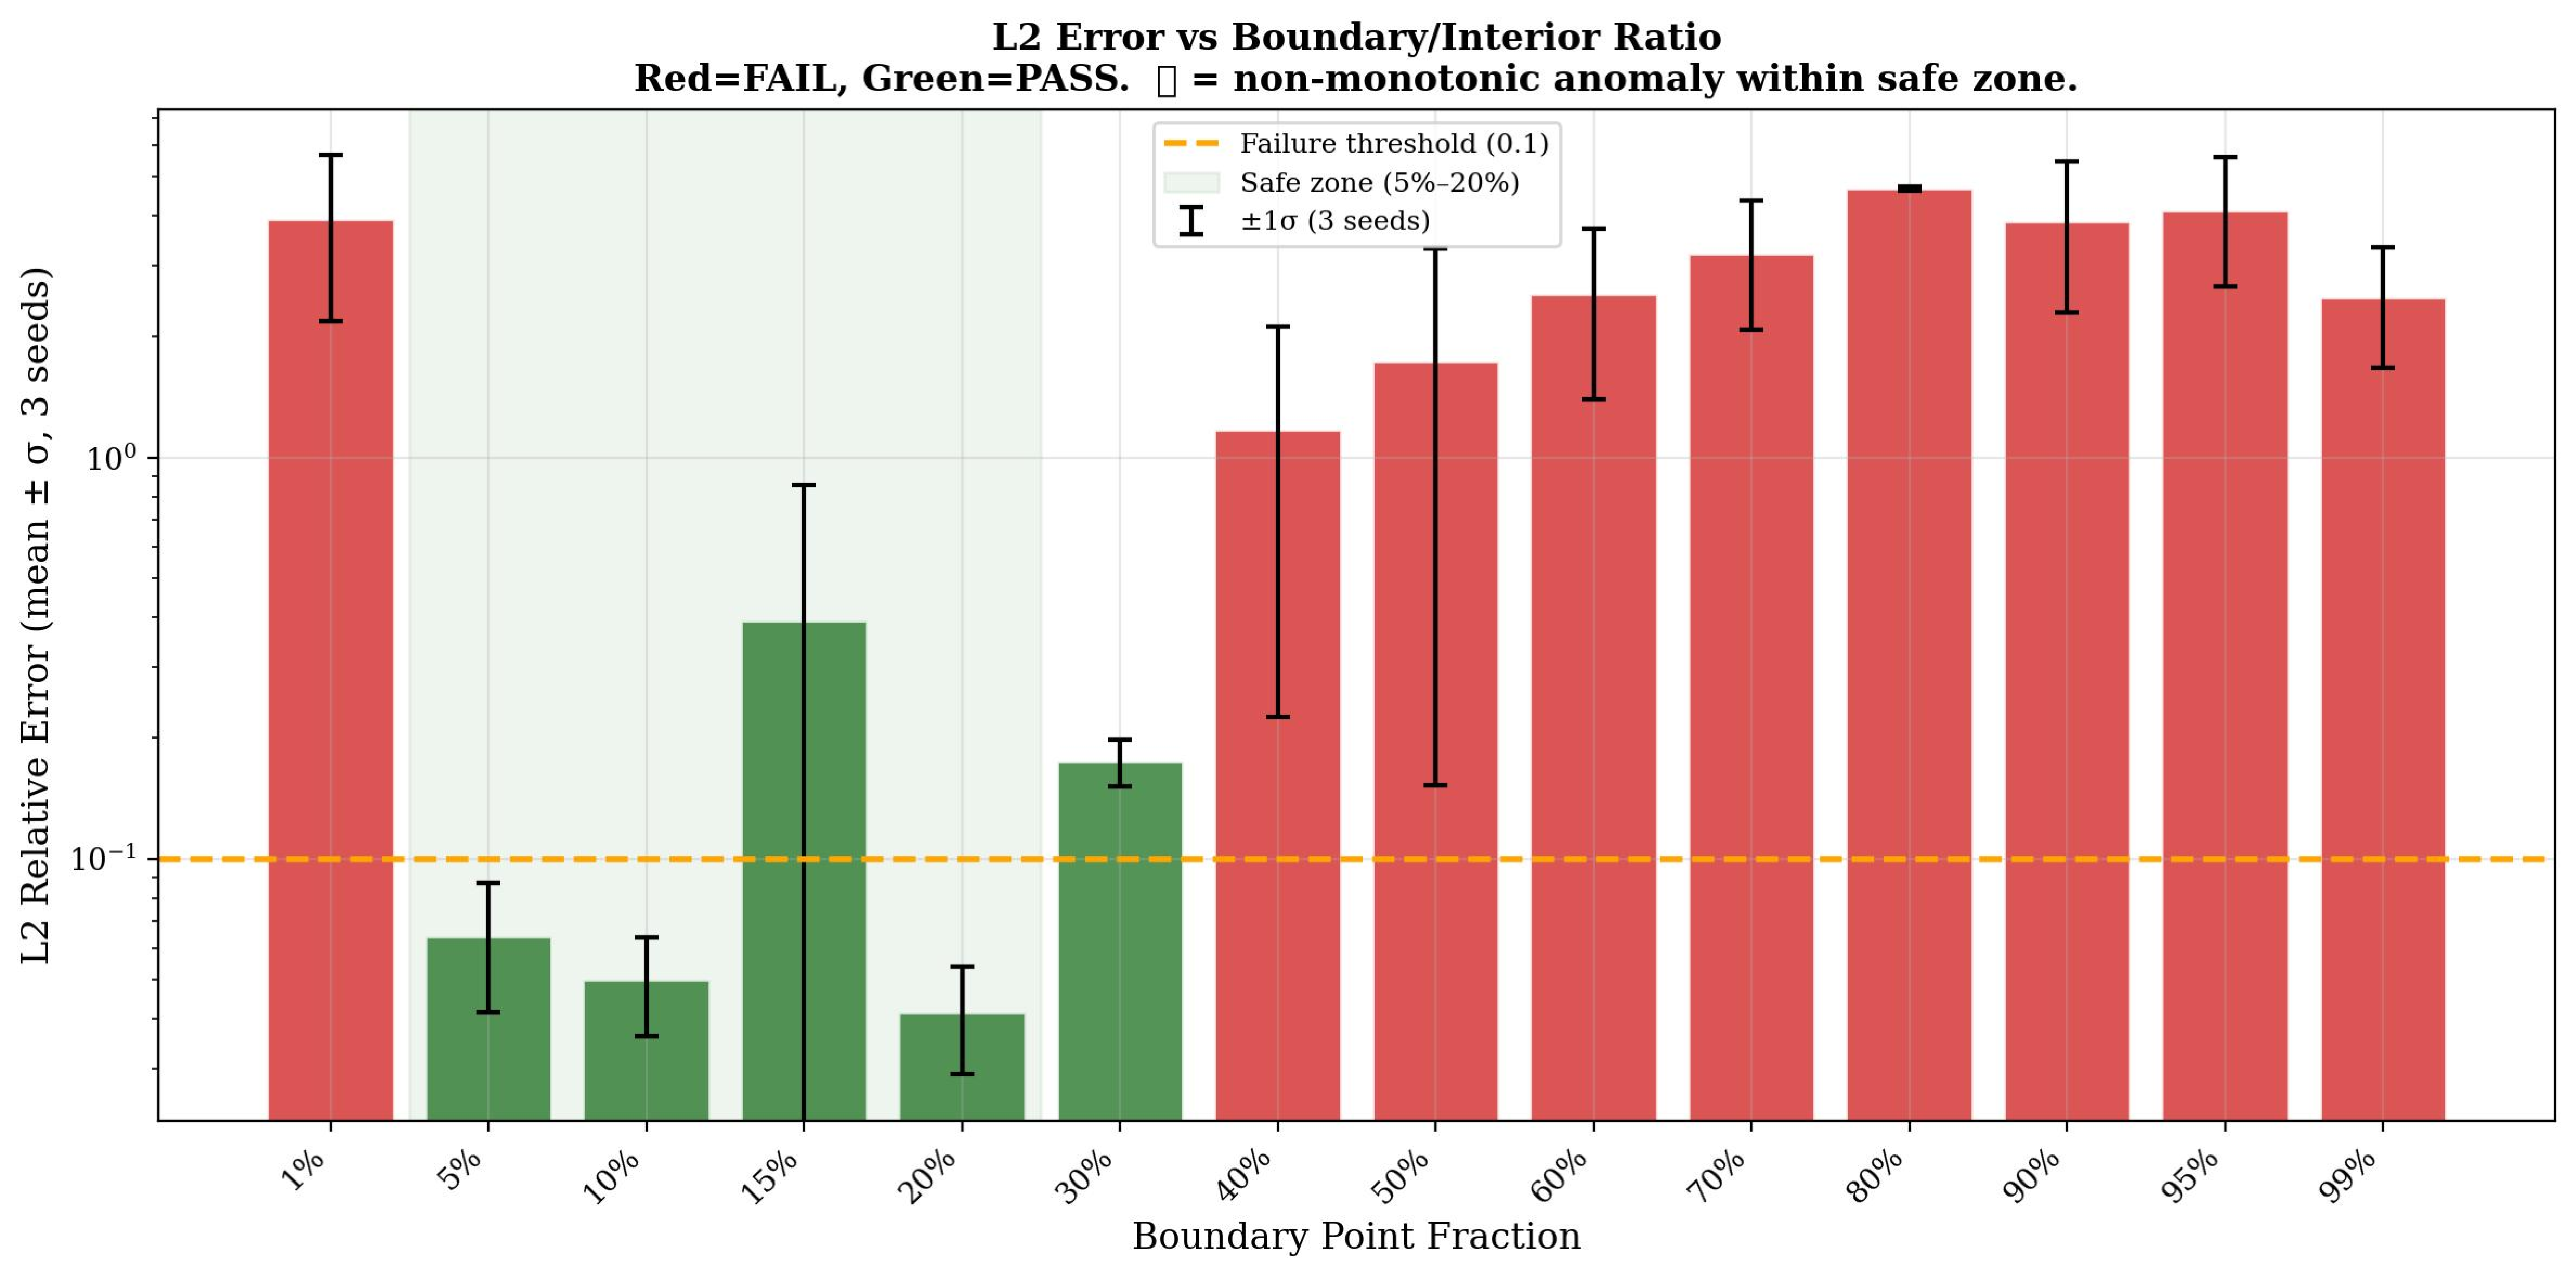
\includegraphics[width=\linewidth]{results/exp9/l2_vs_ratio.pdf}
    \caption{Relative $\Ltwo$ error as a function of the boundary-to-interior point ratio. The safe convergence zone is narrow and bounded strictly between $5\%$ and $30\%$.}
    \label{fig:exp9_ratio}
\end{figure}

\subsection{Experiments 10 \& 11: Operator Sensitivity — Parabolic vs Multi-Scale}\label{sec:exp10}\label{sec:exp11}

To contextualize the failures observed under stiff advection, we analyzed PINN behavior on strictly parabolic (Heat equation, Experiment 10) and multi-scale interface (Allen-Cahn, Experiment 11) problems. Both experiments represent genuine non-failure findings, demonstrating that catastrophic collapse is tightly bound to advective operators.

For the Heat equation, all tested diffusion coefficients $\alpha \in \{1.0, \dots, 0.0001\}$ successfully converged, producing tight $\Ltwo$ errors ranging from $0.00021$ to $0.00156$. The principal optimization challenge observed was that extreme temporal stiffness (e.g., $\alpha = 0.001$ and $0.0001$) depressed the corrected stiffness metric ($\alpha \cdot \lambda_{max}$) to $158.39$ and $15.84$, respectively. This flattened the physical dynamics and caused the optimizer to stall, resulting in premature early stopping where the loss plateaued before the full training budget could be exhausted.

Similarly, for the Allen-Cahn equation, all tested interaction widths $\epsilon$ converged flawlessly ($\Ltwo < 0.002$). However, decomposing the error into boundary and bulk regions revealed a distinct pathology precursor. As $\epsilon$ decreased from $0.1$ to $0.0001$, the interface-to-bulk error ratio steadily climbed from $0.711$ up to $2.698$, indicating that the interface error grows disproportionately faster than the bulk error. The heat equation's dissipative structure aligns with the network's spectral bias, preventing failure. The Allen-Cahn interface narrows as $\epsilon$ decreases, creating a spectral bias precursor visible in the error decomposition even in the absence of global $\Ltwo$ failure.

\begin{figure}[htpb]
    \centering
    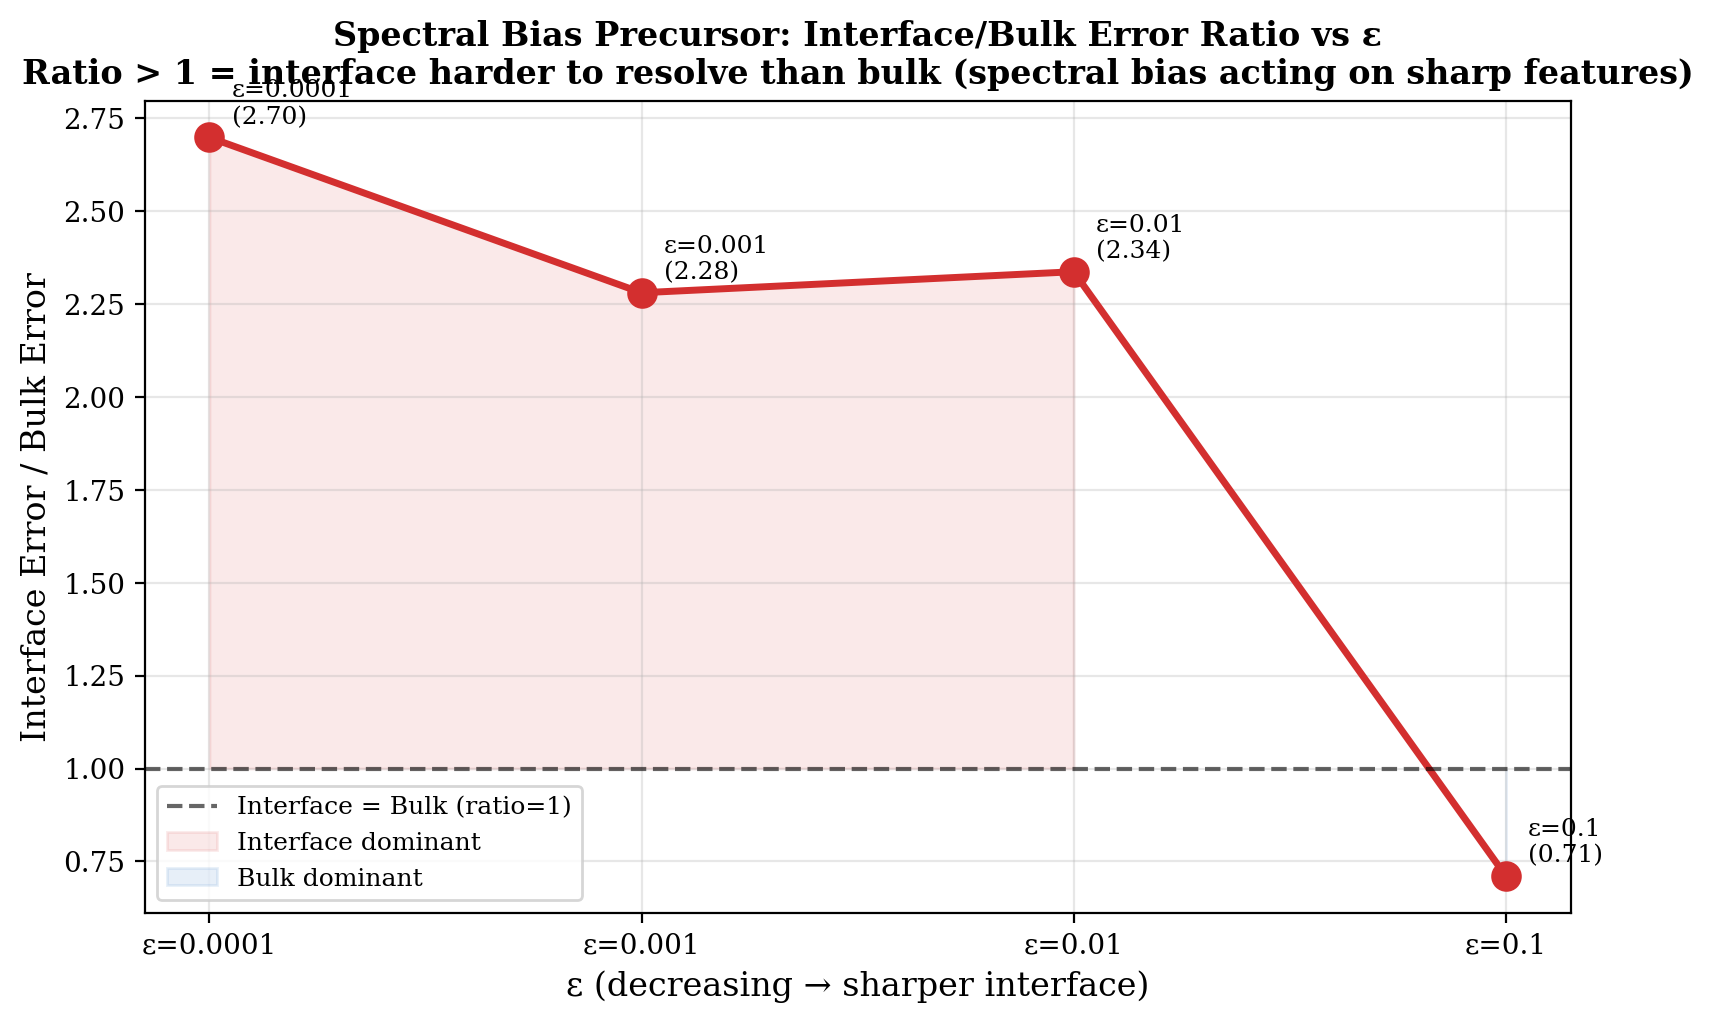
\includegraphics[width=\linewidth]{results/exp11/interface_ratio_trend.png}
    \caption{Interface-to-bulk error ratio as a function of $\epsilon$ for the Allen-Cahn equation, illustrating the emergence of spectral bias.}
    \label{fig:exp11_interface}
\end{figure}

\subsection{Experiment 12: Long-Time Integration}\label{sec:exp12}

Long-time integration of PDEs using PINNs is frequently addressed via temporal windowing. We evaluated a 10-window sequential training protocol against a single-domain baseline over $T \in [0, 10]$. The single domain achieved a peak relative $\Ltwo$ error of $0.0020$, heavily damping high-frequency components but maintaining global stability. The windowed protocol exhibited significantly degraded stability, yielding a peak $\Ltwo$ error of $0.1284$. While the windowed error is objectively larger, both approaches demonstrated continuous polynomial error growth over time ($R^2 = 0.887$ for the single domain, $R^2 = 0.968$ for the windowed protocol).

The windowed training protocol used exact analytical initial conditions at each window boundary rather than model-predicted values. This oracle design represents a best-case scenario for windowed training; error propagation from model outputs would be expected to produce different results. Consequently, we explicitly note that the windowing penalty observed here isolatingly measures the optimization friction of re-initializing the solver, not the cascaded error accumulation of a genuine autoregressive rollout.

\begin{figure}[htpb]
    \centering
    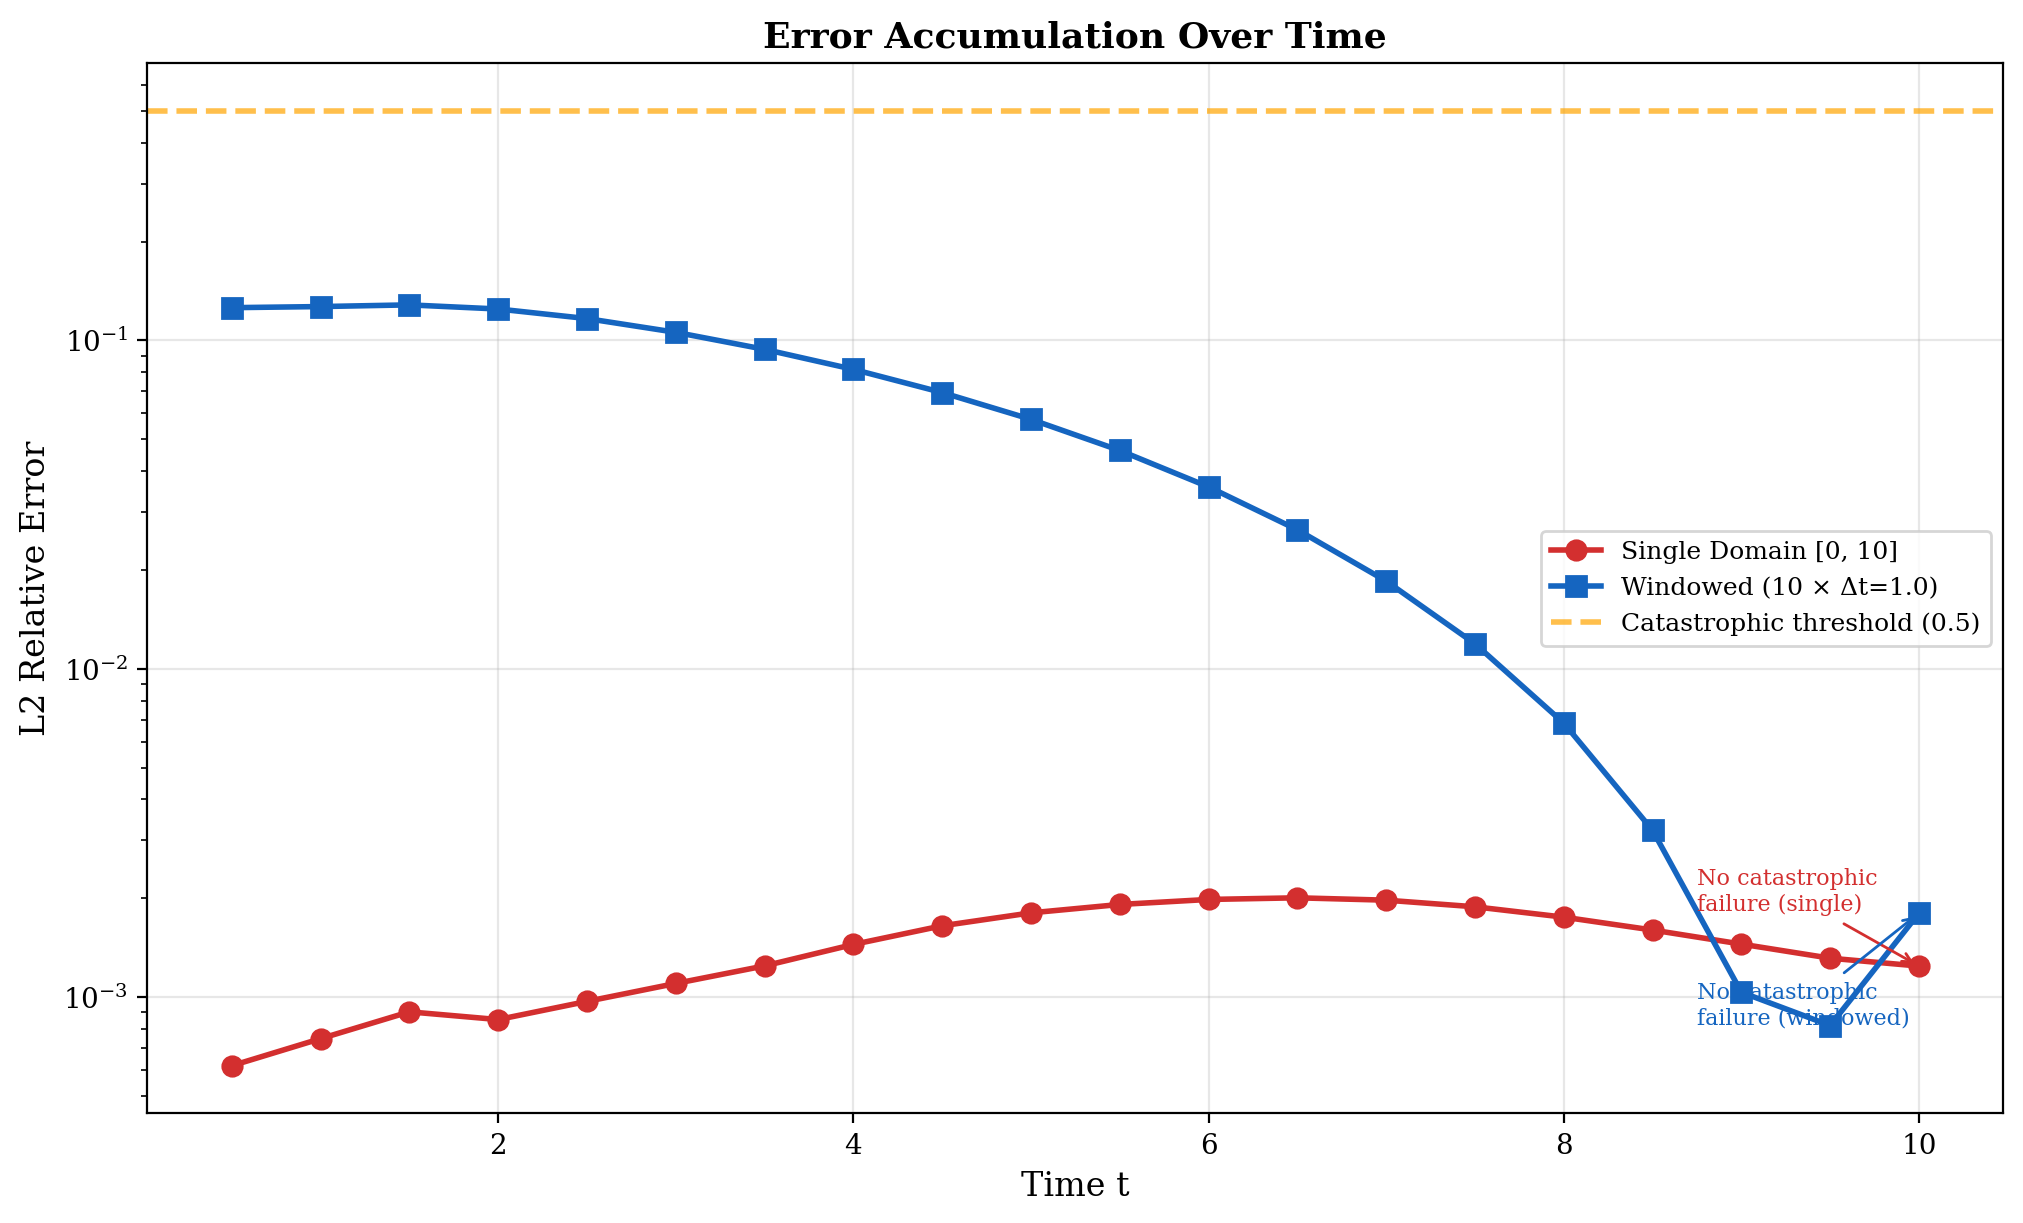
\includegraphics[width=\linewidth]{results/exp12/error_over_time.png}
    \caption{Temporal error growth for single-domain vs windowed long-time integration.}
    \label{fig:exp12_longtime}
\end{figure}

\subsection{Experiment 17: Temporal Extrapolation Horizon}\label{sec:exp17}

Finally, we analyzed the capacity of the standard PINN architecture to extrapolate outside of its training temporal domain, $T_{train}$. We assessed the error at the immediate boundary ($L2_{in}$) and strictly outside the domain ($L2_{out}$), alongside the normalized crossing horizon $R^* = T_{cross} / T_{train}$, where $T_{cross}$ denotes the time the error exceeds $10\%$.

\begin{table}[htpb]
    \centering
    \caption{Temporal extrapolation performance across varied training horizons.}
    \label{tab:exp17_extrapolation}
    \begin{tabular}{@{}lrrrr@{}}
        \toprule
        $T_{train}$ & $L2_{in}$ & $L2_{out}$ & $T_{cross}(10\%)$ & $R^*$ \\
        \midrule
        0.5 & 0.002 & 0.750 & 0.63 & 1.26 \\
        1.0 & 0.001 & 1.726 & 1.18 & 1.18 \\
        2.0 & 0.071 & 1.200 & 2.01 & 1.00 \\
        \bottomrule
    \end{tabular}
\end{table}

Extrapolation degrades rapidly, with the error threshold crossed within 0\% to 26\% of the training horizon depending on $T_{train}$. Notably, extrapolation capacity degrades to absolute zero as the training horizon increases: at $T_{train}=0.5$, the network achieves $R^*=1.26$, but at $T_{train}=1.0$, it achieves $R^*=1.00$, indicating immediate boundary collapse. The network cannot generalize the wave mechanics; it merely coasts on local inertia before diverging. Attempts to fit the out-of-domain error trajectory to established continuous growth models (linear, polynomial, and exponential) uniformly failed, with all models yielding $R^2 < 0.36$ for $T_{train}=1.0$. The error does not follow any continuous growth law beyond $T_{train}$; it saturates immediately at values consistent with the trivial attractor, suggesting the model does not extrapolate but rather snaps to its failure mode. The structural stiffness explicitly confines the network's predictive capabilities strictly to the interpolated convex hull of its collocation data.

\begin{figure}[htpb]
    \centering
    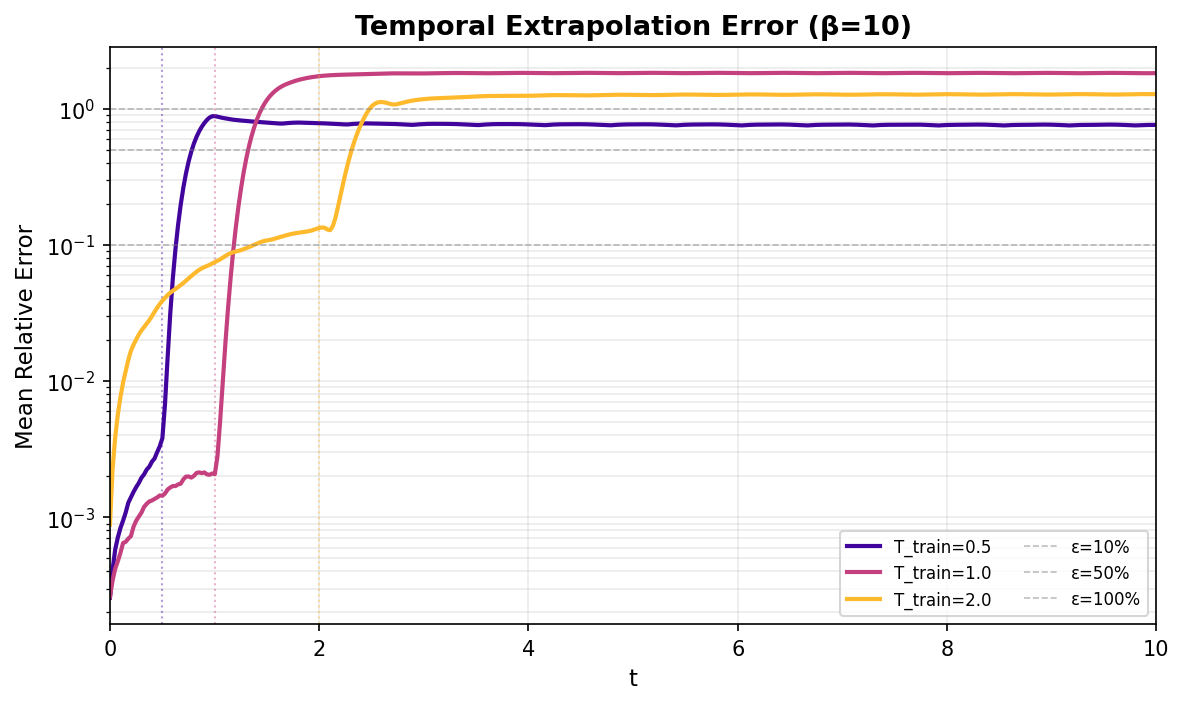
\includegraphics[width=\linewidth]{results/exp17/error_vs_time.png}
    \caption{Extrapolation error drastically breaking the $10\%$ threshold immediately past the $T_{train}$ boundary.}
    \label{fig:exp17_extrap}
\end{figure}

\subsection{Synthesis}

The experiments detailed in this section demonstrate that data sampling strategies—whether through collocation density, boundary enforcement ratios, or temporal domains—cannot fundamentally overcome the structural bottlenecks inherent to standard PINNs on stiff PDEs. Collocation starvation induces uniquely non-monotonic failure landscapes where low training loss falsely implies convergence, while boundary fraction imbalances severely restrict the safe operating envelope. Furthermore, temporal boundaries rigidly trap the network's predictive validity within the interpolated domain, preventing any meaningful extrapolation. A limitation of these data-centric investigations is that they focus strictly on uniform or standard quasi-random sampling within continuous spatial domains; the interaction between geometric stiffness and more advanced, PDE-aware adaptive collocation strategies remains to be fully mapped.
